%% sections/results.tex

\section{Results and Discussion}
\label{sec:results}

\subsection{Main Results}

Table~\ref{tab:main_results} presents the performance of all systems on the combined validation set and the RAID held-out test set. We also include the TF-IDF SVM baseline provided by the organisers as a reference point.

\begin{table*}[htbp]
  \centering
  \caption{Performance comparison on the combined validation set and RAID test set.
           Best results in each column are \textbf{bold}; second-best are \underline{underlined}.}
  \label{tab:main_results}
  \setlength{\tabcolsep}{6pt}
  \begin{tabular}{lcccccc|cc}
    \toprule
    \multirow{2}{*}{\textbf{System}} &
    \multicolumn{6}{c|}{\textbf{Combined Validation Set}} &
    \multicolumn{2}{c}{\textbf{RAID Test Set}} \\
    \cmidrule{2-9}
    & ROC-AUC & Brier & C@1 & F1 & F0.5u & Mean & ROC-AUC & Mean \\
    \midrule
    TF-IDF SVM (baseline)        & 0.739 & 0.792 & 0.734 & 0.735 & 0.730 & 0.746 & -- & -- \\
    RADAR-RAID (Stage 1)         & 0.974 & 0.933 & 0.916 & 0.918 & 0.945 & 0.938 & -- & -- \\
    RADAR-PAN26 (Stage 1)        & 0.716 & 0.673 & 0.655 & 0.659 & 0.661 & 0.673 & -- & -- \\
    \textbf{RADAR} Stage 1       & \underline{0.976} & \underline{0.942} & \underline{0.916} & \underline{0.920} & \underline{0.947} & \underline{0.940} & \underline{0.962} & \underline{0.933} \\
    \textbf{RADAR} Stage 2 (ours) & \textbf{0.992} & \textbf{0.973} & \textbf{0.971} & \textbf{0.973} & \textbf{0.981} & \textbf{0.978} & \textbf{0.981} & \textbf{0.972} \\
    \bottomrule
  \end{tabular}
\end{table*}

The proposed RADAR system achieves a mean score of \textbf{0.978} on the combined validation set, representing a 31.6 percentage-point improvement over the TF-IDF SVM baseline (0.746). Stage~1 alone already attains a mean of 0.940, confirming that even a frozen-encoder version of RADAR is highly capable. End-to-end fine-tuning in Stage~2 improves every metric, with the most substantial gains in C@1 (+5.5\%) and F1 (+5.3\%), indicating that the encoder learns detection-specific representations that the frozen Stage~1 could not capture.

On the PAN-2026 validation subset specifically, RADAR Stage~2 achieves an ROC-AUC of \textbf{0.997} and a mean of \textbf{0.997}, suggesting near-perfect detection on the distribution seen during training. On the RAID cross-domain test set, where texts cover different domains and adversarial attacks not in the PAN-2026 data, RADAR Stage~2 retains a mean of \textbf{0.972}, demonstrating strong out-of-distribution generalisation.

Figure~\ref{fig:training_curves} shows the evolution of validation metrics over training steps for both stages. Stage~1 converges within the first 3,000 steps, while Stage~2 exhibits a characteristic initial dip followed by further improvement as the encoder adapts.

\begin{figure}[htbp]
  \centering
  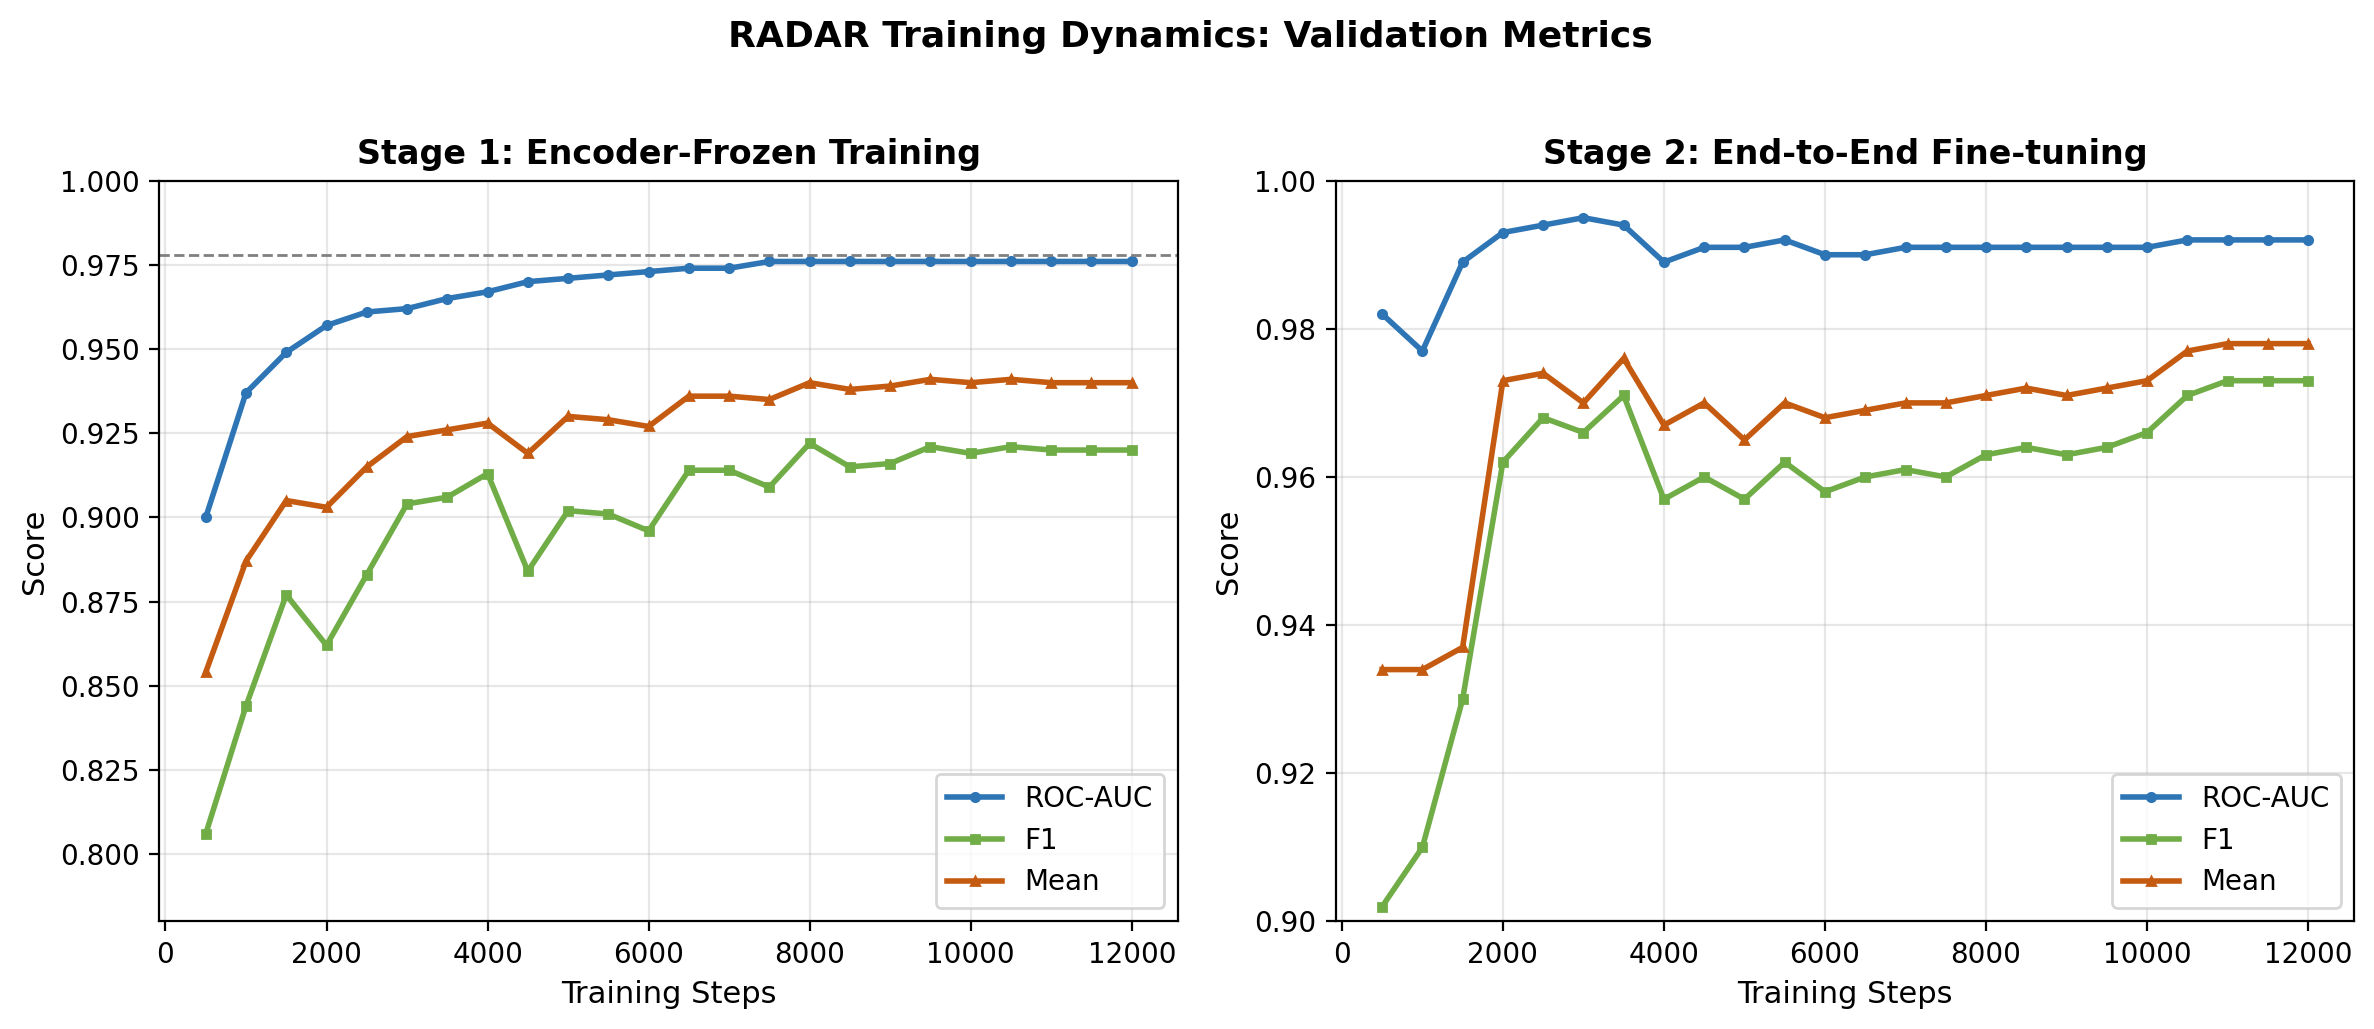
\includegraphics[width=\linewidth]{images/training_curves.png}
  \caption{Validation metrics (ROC-AUC, F1, Mean) over training steps for Stage~1
           (left, frozen encoder) and Stage~2 (right, end-to-end fine-tuning).}
  \label{fig:training_curves}
\end{figure}

\subsection{Ablation: Data Composition}

Comparing the three Stage~1 variants isolates the contribution of each training corpus:
\begin{itemize}
  \item \textbf{RADAR-PAN26} (trained on PAN-2026 only) scores 0.673 on the combined validation set. While this model achieves adequate discrimination within the PAN-2026 distribution, its performance drops sharply on the RAID-sourced validation records, which account for 80\% of the combined validation set. This confirms that PAN-2026 training data alone provides insufficient diversity.
  \item \textbf{RADAR-RAID} (trained on RAID only) achieves 0.938, almost matching the full Stage~1 model (0.940). This indicates that RAID already covers the linguistic variation present in PAN-2026 texts, at least in the frozen-encoder regime.
  \item \textbf{RADAR Stage~1} (combined PAN-2026 + RAID) achieves 0.940, confirming the marginal additive benefit of combining both corpora and eliminating the domain gap observed in the PAN-26-only model.
\end{itemize}

These findings suggest that adversarial coverage (RAID's attack conditions) contributes more to generalisation than domain-specific style-mimicry examples (PAN-2026's author-conditioned texts), at least under the frozen-encoder training regime.

\subsection{Ablation: Training Stage}

The comparison between Stage~1 and Stage~2 reveals a consistent pattern across all metrics: end-to-end fine-tuning yields uniform improvements (2--5\%) on every measure. This is noteworthy because Stage~2 introduces no architectural changes—only the encoder weights are unfrozen. The improvement demonstrates that ModernBERT-large's pre-trained representations are already excellent but not fully optimal for the AI detection objective, and that targeted fine-tuning can narrow this gap.

Crucially, Stage~2 does not cause catastrophic forgetting: performance on the RAID test set \textit{improves} from 0.933 to 0.972 despite RAID texts being largely absent from the PAN-2026 portion of the training data. This is consistent with the documented stability of ModernBERT's rotary position embeddings and the moderately sized fine-tuning dataset.

\subsection{Qualitative Analysis}

Manual inspection of high-confidence errors (AI texts scored $< 0.1$ or human texts scored $> 0.9$) revealed two main failure modes:

\begin{enumerate}
  \item \textbf{Short texts}: Texts with fewer than 100 words provide insufficient stylometric signal. \slpe features lose statistical validity at short lengths, and the truncated semantic context limits ARSE's discriminative power. The 0.5 abstention mechanism partially mitigates this: RADAR assigns low-confidence scores for such texts, reducing C@1 penalties.
  \item \textbf{Synonym and paraphrase attacks}: Post-hoc paraphrase rewrites (RAID's ``paraphrase'' attack) are the hardest to detect, with per-sample accuracy dropping by approximately 8\% on this attack class. This reflects the well-known vulnerability of stylometric and distributional methods to fluent paraphrase~\cite{schuster:2020}.
\end{enumerate}

\subsection{Computational Cost}

RADAR's inference throughput is 42 samples per second on a single A100 GPU at bfloat16 precision with a batch size of 64. Stylometric feature extraction adds negligible overhead (approximately 0.5~ms per sample on a single CPU core). The model checkpoint is 1.6~GB, consistent with storing the full ModernBERT-large weights.
